\documentclass[12pt,a4paper]{report}

% ==============================================================================
% PAQUETES Y CONFIGURACIÓN GENERAL
% ==============================================================================
\usepackage[utf8]{inputenc}
\usepackage[T1]{fontenc}
\usepackage[spanish,es-tabla]{babel}
\usepackage{geometry}
\geometry{top=2.5cm, bottom=2.5cm, left=3.0cm, right=2.5cm}

\usepackage{graphicx}
\usepackage{float}
\usepackage{booktabs}
\usepackage{longtable}
\usepackage{tabularx}
\usepackage{array}
\usepackage{xcolor}
\usepackage{colortbl}
\usepackage{amsmath,amssymb}
\usepackage{fancyhdr}
\usepackage{titlesec}
\usepackage{enumitem}
\usepackage{tcolorbox}
\usepackage{hyperref}

% Configuración de colores institucionales y de estilo
\definecolor{primaryBlue}{RGB}{24, 76, 120}
\definecolor{secondaryBlue}{RGB}{41, 128, 185}
\definecolor{darkGray}{RGB}{60, 64, 67}
\definecolor{lightGray}{RGB}{245, 247, 250}
\definecolor{borderGray}{RGB}{209, 213, 219}
\definecolor{alertRed}{RGB}{192, 57, 43}
\definecolor{accentGreen}{RGB}{39, 174, 96}

% Configuración de hipervínculos
\hypersetup{
    colorlinks=true,
    linkcolor=primaryBlue,
    citecolor=secondaryBlue,
    filecolor=primaryBlue,
    urlcolor=secondaryBlue,
    pdftitle={Especificación de Casos de Uso - SGO},
    pdfauthor={Omar Figueroa, Alexander Villalva},
    pdfsubject={Ingeniería de Software - ESPOCH},
    pdfkeywords={Casos de Uso, UML, PMOInformatica, Optometría, SGO, SRI, Scrum}
}

% Configuración de encabezados y pies de página
\pagestyle{fancy}
\fancyhf{}
\fancyhead[L]{\small\color{darkGray}Sistema de Gestión Optométrica (SGO) — Casos de Uso}
\fancyhead[R]{\small\color{darkGray}Óptica de Estudio}
\fancyfoot[L]{\small\color{darkGray}ESPOCH — Carrera de Software}
\fancyfoot[R]{\thepage}
\renewcommand{\headrulewidth}{0.5pt}
\renewcommand{\footrulewidth}{0.5pt}

% Formato de títulos
\titleformat{\chapter}[display]
  {\normalfont\bfseries\color{primaryBlue}}
  {\filleft\Large\textsf{CAPÍTULO} \Huge\thechapter}
  {1ex}
  {\titlerule[1.5pt]\vspace{1.5ex}\filright\huge}
  [\vspace{1.5ex}\titlerule]

\titleformat{\section}
  {\normalfont\Large\bfseries\color{primaryBlue}}
  {\thesection}{1em}{}

\titleformat{\subsection}
  {\normalfont\large\bfseries\color{secondaryBlue}}
  {\thesubsection}{1em}{}

% Comandos personalizados para tablas estilo PMOInformatica
\newcolumntype{L}[1]{>{\raggedright\let\newline\\\arraybackslash\hspace{0pt}}m{#1}}
\newcolumntype{C}[1]{>{\centering\let\newline\\\arraybackslash\hspace{0pt}}m{#1}}
\newcolumntype{R}[1]{>{\raggedleft\let\newline\\\arraybackslash\hspace{0pt}}m{#1}}

% ==============================================================================
% COMIENZO DEL DOCUMENTO
% ==============================================================================
\begin{document}

% ------------------------------------------------------------------------------
% PORTADA INSTITUCIONAL
% ------------------------------------------------------------------------------
\begin{titlepage}
    \centering
    \vspace*{-1cm}
    
    % Logos institucionales
    \begin{figure}[H]
        \centering
        \begin{minipage}{0.45\textwidth}
            \centering
            % IMAGEN: Logotipo de la ESPOCH
            % Guardar como: pictures/logo_espoch.png en Overleaf
            \includegraphics[height=2.2cm]{pictures/logo_espoch.png}
        \end{minipage}
        \hfill
        \begin{minipage}{0.45\textwidth}
            \centering
            % IMAGEN: Logotipo de Óptica de Estudio
            % Guardar como: pictures/logo_optica_estudio.png en Overleaf
            \includegraphics[height=2.0cm]{pictures/logo_optica_estudio.png}
        \end{minipage}
    \end{figure}
    
    \vspace{0.8cm}
    {\Large\textbf{\color{primaryBlue}ESCUELA SUPERIOR POLITÉCNICA DE CHIMBORAZO}}\\[0.2cm]
    {\large\textbf{FACULTAD DE INFORMÁTICA Y ELECTRÓNICA}}\\[0.15cm]
    {\large\textbf{CARRERA DE SOFTWARE}}\\[0.8cm]
    
    \rule{\linewidth}{1.5pt}\\[0.4cm]
    {\LARGE\textbf{\color{primaryBlue}DOCUMENTO MAESTRO DE ESPECIFICACIÓN}}\\
    \vspace{0.2cm}
    {\LARGE\textbf{\color{primaryBlue}DE CASOS DE USO (UML 2.5)}}\\[0.3cm]
    {\large\textbf{SISTEMA INFORMÁTICO DE GESTIÓN CLÍNICA Y COMERCIAL OPTOMÉTRICA (SGO)}}\\[0.2cm]
    {\normalsize\textit{Estandarizado conforme a la Plantilla de Casos de Uso de PMOInformática,\\normas ISO/IEC 25010:2023 y la metodología ágil Secure Scrum}}\\
    \rule{\linewidth}{1.5pt}\\[1.0cm]
    
    \begin{minipage}{0.48\textwidth}
        \textbf{Autores / Investigadores:}\\[0.15cm]
        Omar Santiago Figueroa Díaz\\
        \textit{C.I. 1803391968 --- Código: 7253}\\[0.2cm]
        Alexander Rafael Villalva Dumancela\\
        \textit{C.I. 0605351899 --- Código: 7135}
    \end{minipage}
    \hfill
    \begin{minipage}{0.48\textwidth}
        \raggedleft
        \textbf{Director / Tutor Académico:}\\[0.15cm]
        Ing. Jorge Ariel Menéndez Verdecia\\[0.3cm]
        \textbf{Entidad Beneficiaria:}\\[0.15cm]
        Óptica de Estudio\\
        \textit{Riobamba, Chimborazo, Ecuador}
    \end{minipage}
    
    \vfill
    {\large\textbf{Riobamba --- Ecuador}}\\[0.2cm]
    {\normalsize Septiembre de 2026 --- Versión 1.0 Definitiva}
\end{titlepage}

% ------------------------------------------------------------------------------
% HISTORIAL DE VERSIONES, APROBACIONES E ÍNDICE
% ------------------------------------------------------------------------------
\newpage
\chapter*{Control Documental y Aprobaciones}
\addcontentsline{toc}{chapter}{Control Documental y Aprobaciones}

\section*{Historial de Versiones}
\begin{table}[H]
\centering
\small
\begin{tabularx}{\textwidth}{|c|c|L{4.0cm}|L{3.0cm}|X|}
\hline
\rowcolor{primaryBlue}\color{white}\textbf{Fecha} & \rowcolor{primaryBlue}\color{white}\textbf{Versión} & \rowcolor{primaryBlue}\color{white}\textbf{Autor} & \rowcolor{primaryBlue}\color{white}\textbf{Organización} & \rowcolor{primaryBlue}\color{white}\textbf{Descripción del Cambio} \\
\hline
25/09/2026 & 1.0 & Figueroa Omar, Villalva Alex. & ESPOCH / SGO & Versión definitiva consolidada que integra los 23 casos de uso del sistema bajo estándar PMOInformática. \\
\hline
\end{tabularx}
\caption{Historial formal de versiones del documento.}
\end{table}

\vspace{0.8cm}
\section*{Información del Proyecto}
\begin{table}[H]
\centering
\small
\begin{tabularx}{\textwidth}{|L{5.5cm}|X|}
\hline
\rowcolor{lightGray}\textbf{Empresa / Organización:} & Óptica de Estudio --- Riobamba, Ecuador \\
\hline
\textbf{Proyecto:} & Sistema Informático de Gestión Clínica y Comercial Optométrica (SGO) \\
\hline
\rowcolor{lightGray}\textbf{Fecha de Preparación:} & 25 de Septiembre de 2026 \\
\hline
\textbf{Cliente / Stakeholder:} & Optometrista Propietario de Óptica de Estudio \\
\hline
\rowcolor{lightGray}\textbf{Director / Tutor Académico:} & Ing. Jorge Ariel Menéndez Verdecia (ESPOCH) \\
\hline
\textbf{Líderes de Proyecto / Desarrollo:} & Alexander Rafael Villalva Dumancela / Omar Santiago Figueroa Díaz \\
\hline
\end{tabularx}
\caption{Metadatos de identificación del proyecto.}
\end{table}

\vspace{0.8cm}
\section*{Acta Formal de Aprobaciones}
\begin{table}[H]
\centering
\small
\begin{tabularx}{\textwidth}{|L{4.2cm}|L{3.5cm}|L{3.2cm}|c|c|}
\hline
\rowcolor{primaryBlue}\color{white}\textbf{Nombre y Apellido} & \rowcolor{primaryBlue}\color{white}\textbf{Cargo} & \rowcolor{primaryBlue}\color{white}\textbf{Institución} & \rowcolor{primaryBlue}\color{white}\textbf{Fecha} & \rowcolor{primaryBlue}\color{white}\textbf{Firma} \\
\hline
Ing. Jorge Menéndez Verdecia & Director de Titulación & Carrera Software ESPOCH & 25/09/2026 & [Aprobado] \\
\hline
Alexander Villalva Dumancela & Líder de Proyecto & Equipo Investigador & 25/09/2026 & [Aprobado] \\
\hline
Omar Santiago Figueroa Díaz & Líder de Software & Equipo Investigador & 25/09/2026 & [Aprobado] \\
\hline
Lic. Optometrista Titular & Propietario / Cliente & Óptica de Estudio & 25/09/2026 & [Aprobado] \\
\hline
\end{tabularx}
\caption{Firmas de homologación académica y técnica.}
\end{table}

\newpage
\tableofcontents
\listoffigures
\listoftables

% ==============================================================================
% CAPÍTULO 1: RESUMEN EJECUTIVO Y ALCANCE
% ==============================================================================
\newpage
\chapter{Resumen Ejecutivo y Alcance del Sistema}

\section{Introducción y Alcance Global}
El presente documento constituye la especificación canónica y exhaustiva de los Casos de Uso (CU) del \textbf{Sistema Informático de Gestión Clínica y Comercial Optométrica (SGO)}. El propósito medular del sistema es resolver de manera automatizada, integral y segura la gestión de la atención visual, los flujos de graduación óptica, el encargo técnico a laboratorios externos de biselado, la facturación electrónica bajo normativa del Servicio de Rentas Internas (SRI) del Ecuador y el control comercial de mostrador en el establecimiento \textbf{Óptica de Estudio} (Riobamba, Ecuador).

\section{Estructura Modular del Sistema (M1 a M7)}
El sistema modela 23 Casos de Uso funcionales organizados jerárquicamente en 7 subsistemas o paquetes:
\begin{enumerate}[label=\textbf{M\arabic*:}, leftmargin=1.5cm]
    \item \textbf{Gestión de Acceso y Seguridad RBAC:} Control criptográfico de autenticación con Argon2id, tokens JWT RS256 y caducidad por inactividad.
    \item \textbf{Gestión Demográfica de Pacientes:} Filiación formal con validador algorítmico Módulo 10 para cédulas ecuatorianas, gestión pediátrica y búsqueda predictiva.
    \item \textbf{Atención Clínica y Refracción Integral:} Anamnesis estructurada, lensometría de gafas previas, queratometría computarizada, refracción subjetiva, validación de marcha y control patológico de pterigión.
    \item \textbf{Taller y Laboratorio Óptico:} Emisión de órdenes disociadas bajo LOPDP, instrucciones milimétricas de biselado en armazones semialaire y trazabilidad de pedidos.
    \item \textbf{Ventas, Caja y Mostrador:} Cotización de combos promocionales mensuales ($99.00 USD), cobro de anticipos con ticket vinculante de retiro, liquidación y arqueo ciego diario.
    \item \textbf{Facturación Electrónica SRI:} Ensamblaje XML v1.1.0, generación de clave de acceso ponderada de 49 dígitos (Módulo 11), firma digital XAdES-BES en PKCS\#12 y contingencia offline.
    \item \textbf{Asistente Inteligente y Auditoría Inmutable:} Consultas en lenguaje natural blindadas con Read-Only Guard (\texttt{GRANT SELECT}) y bitácora criptográfica con Hash Chain (SHA-256).
\end{enumerate}

\section{Integración de Hallazgos Críticos de la Sesión Real (Audio)}
A diferencia de formulaciones preliminares abstractas, la especificación incorpora 6 brechas operativas detectadas en la grabación clínica del 25 de septiembre de 2026:
\begin{itemize}[leftmargin=1.0cm]
    \item \textbf{Lensometría Física Previa (CU-CLI-02):} Medición in situ de la fórmula en uso (+1.75 / -1.50) y diagnóstico de daño físico por astillamiento inferior.
    \item \textbf{Queratometría Computarizada (CU-CLI-03):} Parámetros corneales objetivos K1/K2 y cálculo de astigmatismo corneal ($\Delta K = K_2 - K_1$).
    \item \textbf{Test de Marcha Dinámica (CU-CLI-04):} Verificación en aros de prueba de la ausencia de mareos y desniveles en piso antes de sellar la prescripción.
    \item \textbf{Seguimiento de Pterigión (CU-CLI-06):} Mapeo de carnosidad en cara interna nasal (Grado I) con prescripción preventiva de filtro UV400 y advertencia de no frotamiento.
    \item \textbf{Ajuste Geométrico de Biselado (CU-LAB-01):} Reducción vertical milimétrica de montura de 38 mm a 27 mm para aro semialaire con ranurado de nylon.
    \item \textbf{Paquete Promocional y Orden de Retiro (CU-VEN-02 / CU-VEN-03):} Tarifa plana de $99.00 USD, abono inicial de $50 y entrega programada en 2 días laborables (viernes).
\end{itemize}

% ==============================================================================
% CAPÍTULO 2: CATÁLOGO DE ACTORES DEL SISTEMA
% ==============================================================================
\newpage
\chapter{Catálogo Maestro de Actores del Sistema}

Conforme a la metodología de PMOInformática, se presentan las fichas técnicas formales de los actores que interactúan con el SGO:

\section{ACT-00: Usuario Autenticado (Actor Abstracto Base)}
\begin{table}[H]
\centering
\small
\begin{tabularx}{\textwidth}{|L{3.5cm}|X|}
\hline
\rowcolor{primaryBlue}\color{white}\textbf{Campo} & \rowcolor{primaryBlue}\color{white}\textbf{Especificación} \\
\hline
\textbf{Actor:} & Usuario Autenticado \\
\hline
\textbf{Identificador:} & ACT-00 \\
\hline
\textbf{Descripción:} & Generalización abstracta de todo operador humano con credenciales verificadas y sesión activa en el sistema. \\
\hline
\textbf{Características:} & Personal del centro óptico asignado a una terminal. Heredado por ACT-01, ACT-02 y ACT-03. \\
\hline
\textbf{Relación:} & Generalización de ACT-01, ACT-02 y ACT-03. \\
\hline
\textbf{Referencias:} & CU-SEG-01, CU-SEG-02, CU-PAC-03, CU-IA-01. \\
\hline
\end{tabularx}
\caption{Ficha del Actor ACT-00: Usuario Autenticado.}
\end{table}

\begin{table}[H]
\centering
\small
\begin{tabularx}{\textwidth}{|L{4.0cm}|X|c|}
\hline
\rowcolor{lightGray}\textbf{Nombre Atributo} & \textbf{Descripción Funcional} & \textbf{Tipo de Dato} \\
\hline
\texttt{user\_id} & Identificador universal único del usuario & UUID \\
\hline
\texttt{username} & Nombre de cuenta de inicio de sesión & Varchar(50) \\
\hline
\texttt{password\_hash} & Resumen criptográfico de clave en Argon2id & Varchar(255) \\
\hline
\texttt{rol\_id} & Identificador de rol para control de acceso RBAC & Enum / Integer \\
\hline
\texttt{intentos\_fallidos} & Contador de intentos fallidos antes de bloqueo & Smallint \\
\hline
\end{tabularx}
\caption{Atributos del Actor ACT-00.}
\end{table}

\section{ACT-01: Administrador / Propietario}
\begin{table}[H]
\centering
\small
\begin{tabularx}{\textwidth}{|L{3.5cm}|X|}
\hline
\rowcolor{primaryBlue}\color{white}\textbf{Campo} & \rowcolor{primaryBlue}\color{white}\textbf{Especificación} \\
\hline
\textbf{Actor:} & Administrador / Propietario \\
\hline
\textbf{Identificador:} & ACT-01 \\
\hline
\textbf{Descripción:} & Representante legal y máxima autoridad administrativa. Gestiona usuarios, custodia llaves criptográficas de facturación SRI, realiza arqueos y autoriza anulaciones atómicas ACID. \\
\hline
\textbf{Características:} & Privilegios totales de gobierno y auditoría. Hereda de ACT-00. \\
\hline
\textbf{Atributos Clave:} & \texttt{ruc\_establecimiento} (Varchar 13), \texttt{pin\_autorizacion} (Varchar 255), \texttt{email\_alertas} (Varchar 100). \\
\hline
\textbf{Referencias:} & CU-SEG-01, CU-VEN-05, CU-VEN-06, CU-SRI-02, CU-IA-01, CU-AUD-01. \\
\hline
\end{tabularx}
\caption{Ficha del Actor ACT-01: Administrador / Propietario.}
\end{table}

\section{ACT-02: Optometrista Clínico}
\begin{table}[H]
\centering
\small
\begin{tabularx}{\textwidth}{|L{3.5cm}|X|}
\hline
\rowcolor{primaryBlue}\color{white}\textbf{Campo} & \rowcolor{primaryBlue}\color{white}\textbf{Especificación} \\
\hline
\textbf{Actor:} & Optometrista Clínico \\
\hline
\textbf{Identificador:} & ACT-02 \\
\hline
\textbf{Descripción:} & Profesional facultado de la salud visual. Responsable de anamnesis, lensometría, refracción subjetiva, confort en marcha, prescripción y emisión de órdenes de taller. \\
\hline
\textbf{Características:} & Especialista médico habilitado por el MSP con firma digitalizada. Hereda de ACT-00. \\
\hline
\textbf{Atributos Clave:} & \texttt{registro\_msp} (Varchar 25), \texttt{especialidad} (Varchar 100), \texttt{firma\_digital\_id} (UUID). \\
\hline
\textbf{Referencias:} & CU-CLI-01 a CU-CLI-06, CU-LAB-01, CU-PAC-01. \\
\hline
\end{tabularx}
\caption{Ficha del Actor ACT-02: Optometrista Clínico.}
\end{table}

\section{ACT-03: Asistente Comercial / Recepcionista}
\begin{table}[H]
\centering
\small
\begin{tabularx}{\textwidth}{|L{3.5cm}|X|}
\hline
\rowcolor{primaryBlue}\color{white}\textbf{Campo} & \rowcolor{primaryBlue}\color{white}\textbf{Especificación} \\
\hline
\textbf{Actor:} & Asistente Comercial / Recepcionista \\
\hline
\textbf{Identificador:} & ACT-03 \\
\hline
\textbf{Descripción:} & Personal de atención al cliente en mostrador y recepción. Realiza filiación de pacientes, cotización de combos, cobro de anticipos, emisión de órdenes de retiro y entrega. \\
\hline
\textbf{Características:} & Operador ágil de terminal de punto de venta (POS). Hereda de ACT-00. \\
\hline
\textbf{Atributos Clave:} & \texttt{punto\_emision\_pos} (Char 3), \texttt{caja\_sesion\_id} (UUID), \texttt{limite\_descuento} (Numeric 5,2). \\
\hline
\textbf{Referencias:} & CU-PAC-01 a CU-PAC-03, CU-VEN-01 a CU-VEN-04, CU-SRI-01. \\
\hline
\end{tabularx}
\caption{Ficha del Actor ACT-03: Asistente Comercial / Recepcionista.}
\end{table}

\section{ACT-04: Web Services SRI (Actor Externo)}
\begin{table}[H]
\centering
\small
\begin{tabularx}{\textwidth}{|L{3.5cm}|X|}
\hline
\rowcolor{primaryBlue}\color{white}\textbf{Campo} & \rowcolor{primaryBlue}\color{white}\textbf{Especificación} \\
\hline
\textbf{Actor:} & Web Services SRI (Servicio de Rentas Internas) \\
\hline
\textbf{Identificador:} & ACT-04 \\
\hline
\textbf{Descripción:} & Servidores tributarios del Estado ecuatoriano que exponen servicios web SOAP para recepción y autorización de comprobantes electrónicos fuera de línea. \\
\hline
\textbf{Atributos Clave:} & \texttt{url\_recepcion\_soap}, \texttt{url\_autorizacion\_soap}, \texttt{version\_xsd} (1.1.0). \\
\hline
\textbf{Referencias:} & CU-SRI-03. \\
\hline
\end{tabularx}
\caption{Ficha del Actor ACT-04: Web Services SRI.}
\end{table}

\section{ACT-05: Taller Óptico / Laboratorio Externo (Actor Secundario)}
\begin{table}[H]
\centering
\small
\begin{tabularx}{\textwidth}{|L{3.5cm}|X|}
\hline
\rowcolor{primaryBlue}\color{white}\textbf{Campo} & \rowcolor{primaryBlue}\color{white}\textbf{Especificación} \\
\hline
\textbf{Actor:} & Taller Óptico / Laboratorio Externo \\
\hline
\textbf{Identificador:} & ACT-05 \\
\hline
\textbf{Descripción:} & Proveedor tercerizado receptor de la orden técnica de producción para biselado, tallado y tratamiento de lunas sin acceso a datos clínicos del paciente. \\
\hline
\textbf{Atributos Clave:} & \texttt{laboratorio\_id} (UUID), \texttt{razon\_social\_lab} (Varchar 120), \texttt{dias\_entrega} (Smallint). \\
\hline
\textbf{Referencias:} & CU-LAB-01, CU-LAB-02, CU-LAB-03. \\
\hline
\end{tabularx}
\caption{Ficha del Actor ACT-05: Taller Óptico Externo.}
\end{table}

\section{ACT-NEG-01: Paciente / Cliente (Beneficiario Pasivo)}
\begin{table}[H]
\centering
\small
\begin{tabularx}{\textwidth}{|L{3.5cm}|X|}
\hline
\rowcolor{primaryBlue}\color{white}\textbf{Campo} & \rowcolor{primaryBlue}\color{white}\textbf{Especificación} \\
\hline
\textbf{Actor:} & Paciente / Cliente \\
\hline
\textbf{Identificador:} & ACT-NEG-01 \\
\hline
\textbf{Descripción:} & Persona que recibe la atención visual y adquiere insumos. Es el titular de los datos protegidos por la LOPDP y receptor legal de la receta y comprobantes. \\
\hline
\textbf{Referencias:} & CU-CLI-04, CU-CLI-05, CU-VEN-03, CU-VEN-04. \\
\hline
\end{tabularx}
\caption{Ficha del Actor ACT-NEG-01: Paciente / Cliente.}
\end{table}

% ==============================================================================
% CAPÍTULO 3: DIAGRAMA MAESTRO Y MAPA DE PAQUETES
% ==============================================================================
\newpage
\chapter{Diagramas de Casos de Uso y Arquitectura de Paquetes}

\section{Diagrama General de Paquetes UML 2.5}
A continuación se presenta la vista de descomposición modular del sistema SGO:

\begin{figure}[H]
    \centering
    % IMAGEN: Diagrama General de Arquitectura de Paquetes SGO
    % Guardar como: pictures/diagrama_general_paquetes.png en Overleaf
    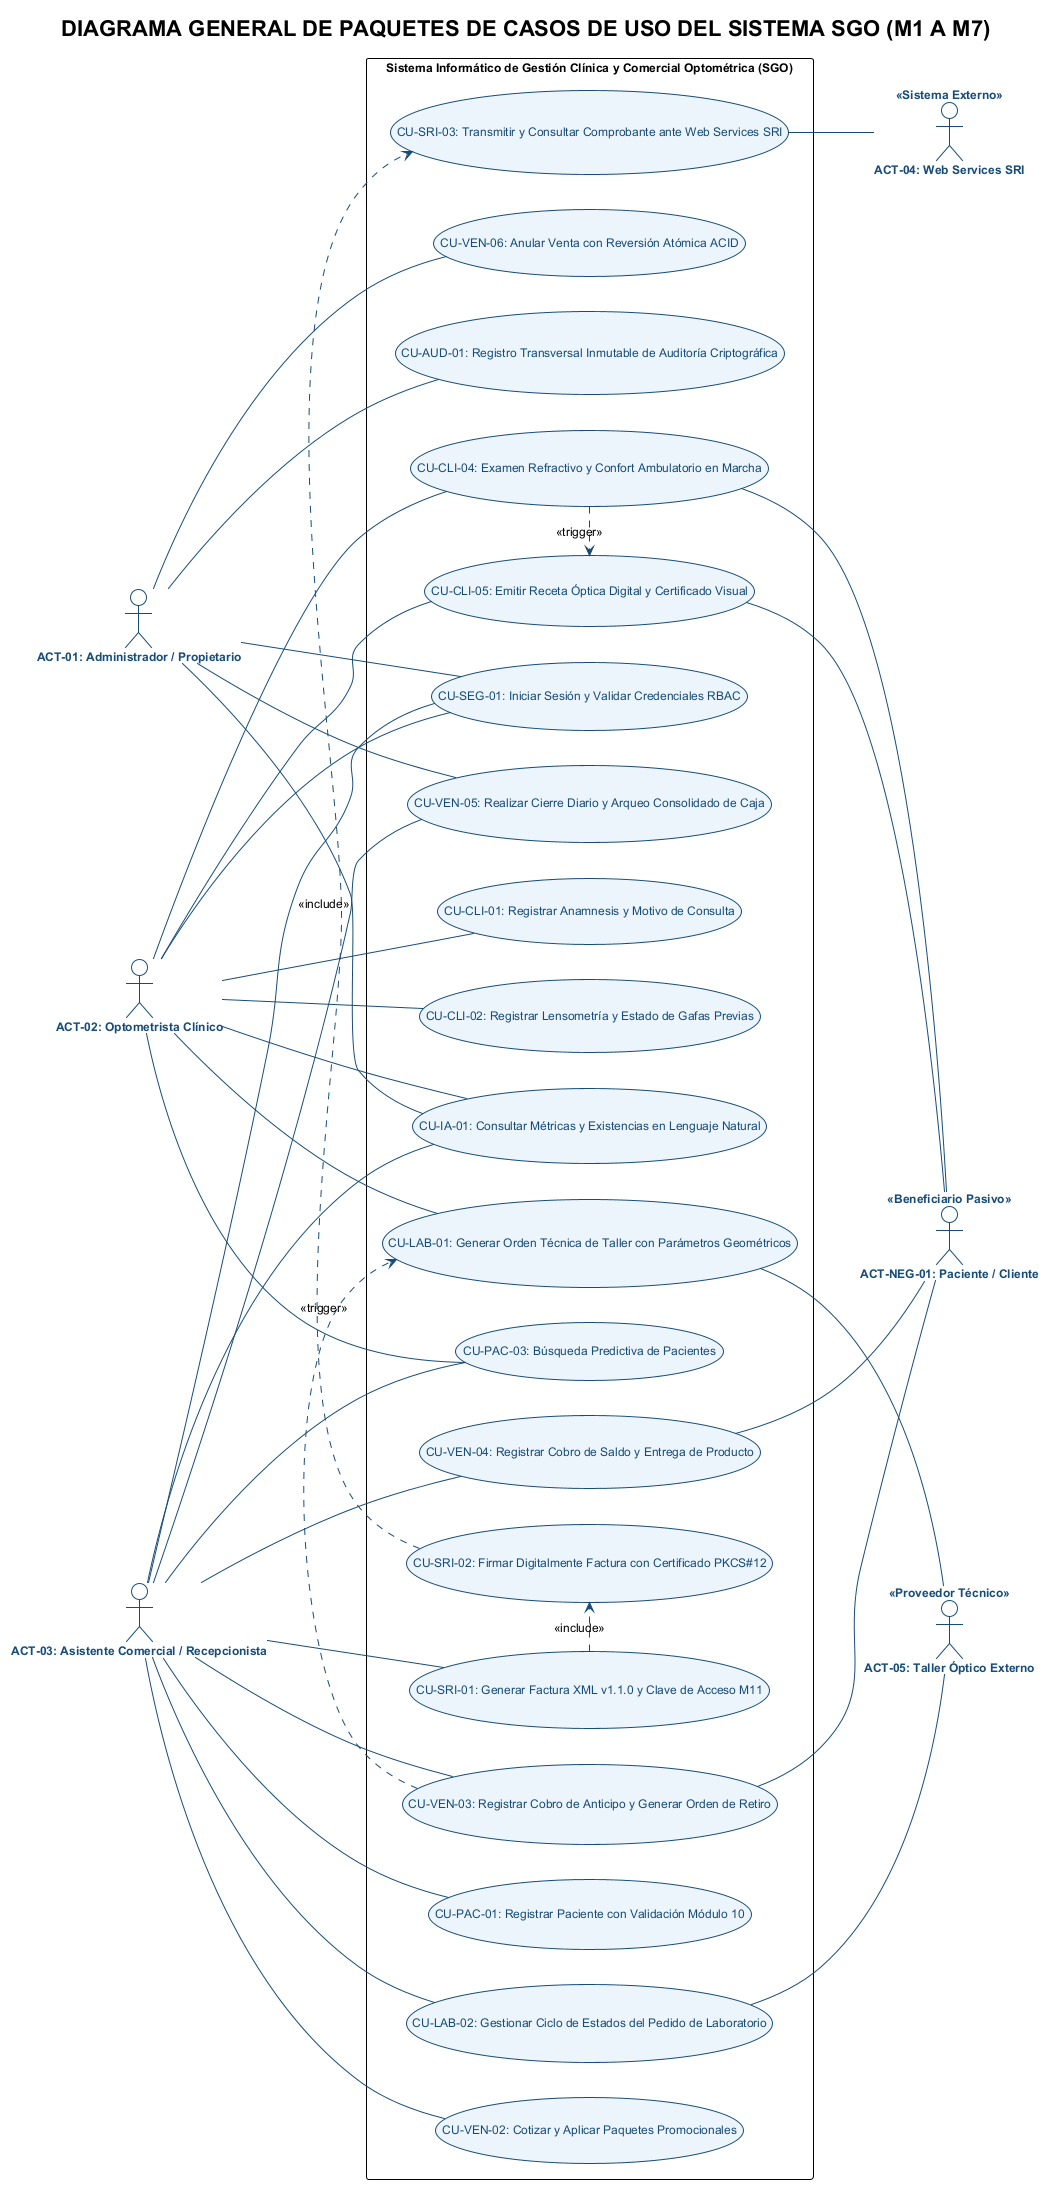
\includegraphics[width=0.92\textwidth]{pictures/diagrama_general_paquetes.png}
    \caption{Diagrama General de Paquetes de Casos de Uso del Sistema SGO (M1 a M7).}
    \label{fig:diagrama_general_paquetes}
\end{figure}

\section{Diagrama de Casos de Uso: Seguridad y Pacientes (M1 y M2)}
\begin{figure}[H]
    \centering
    % IMAGEN: Diagrama de Casos de Uso M1 y M2
    % Guardar como: pictures/diagrama_cu_seguridad_pacientes.png en Overleaf
    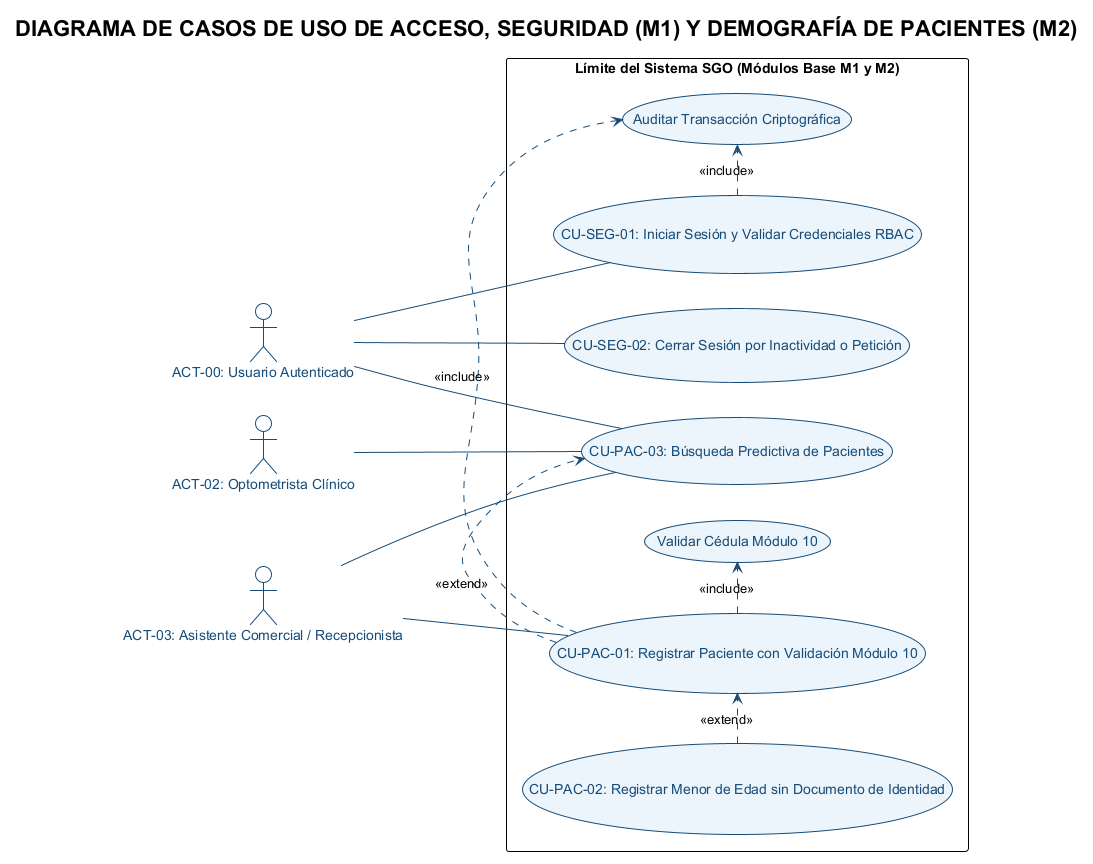
\includegraphics[width=0.88\textwidth]{pictures/diagrama_cu_seguridad_pacientes.png}
    \caption{Diagrama de Casos de Uso de Acceso, Seguridad (M1) y Demografía de Pacientes (M2).}
    \label{fig:diagrama_cu_seguridad_pacientes}
\end{figure}

\section{Diagrama de Casos de Uso: Núcleo Clínico y Refracción (M3)}
\begin{figure}[H]
    \centering
    % IMAGEN: Diagrama de Casos de Uso M3
    % Guardar como: pictures/diagrama_cu_clinico.png en Overleaf
    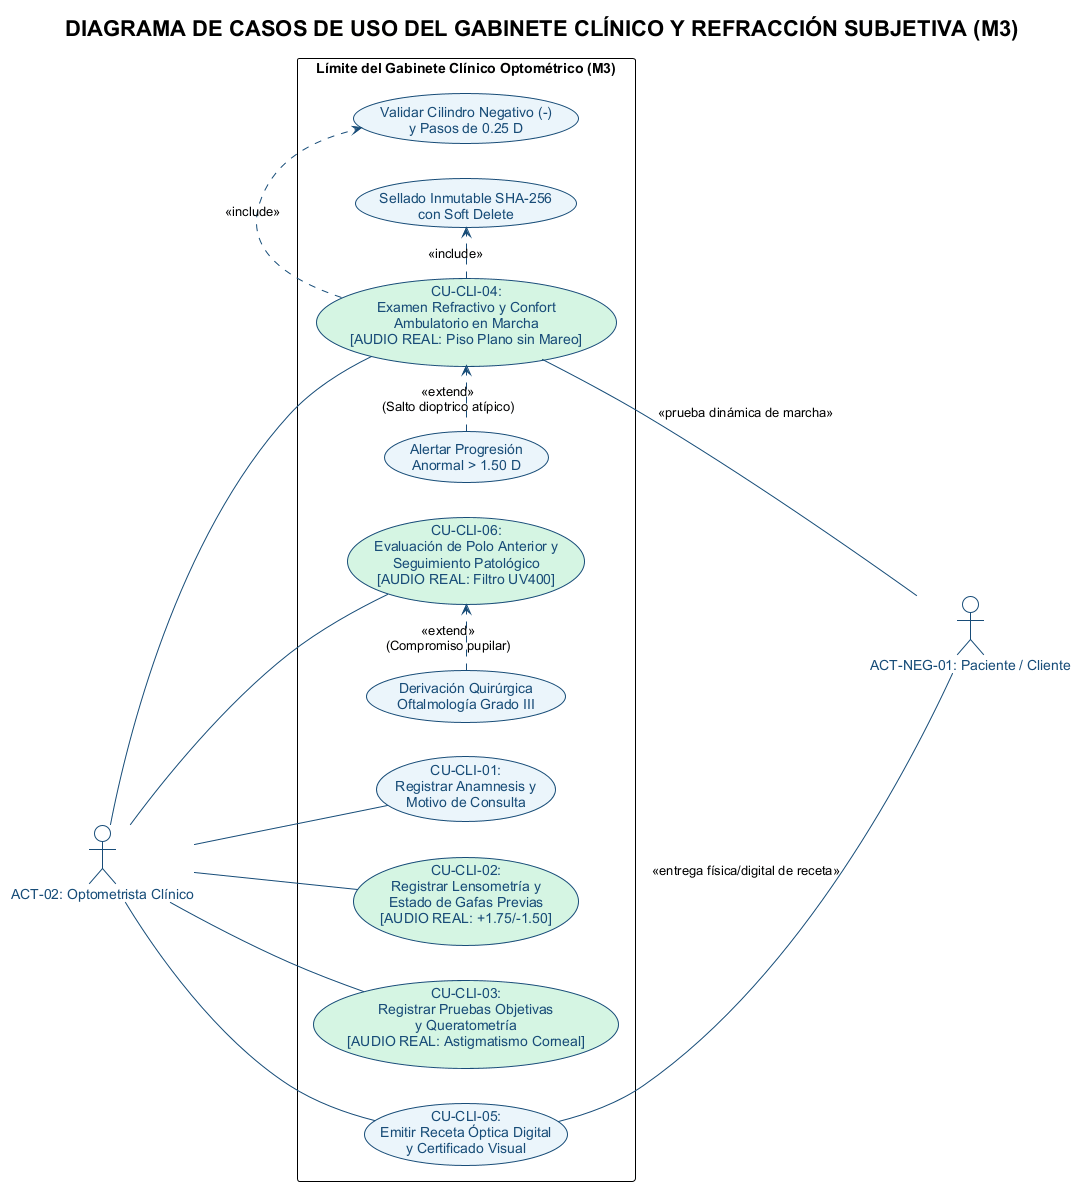
\includegraphics[width=0.88\textwidth]{pictures/diagrama_cu_clinico.png}
    \caption{Diagrama de Casos de Uso del Gabinete Clínico y Refracción Subjetiva (M3).}
    \label{fig:diagrama_cu_clinico}
\end{figure}

\section{Diagrama de Casos de Uso: Taller Óptico, Ventas y Caja (M4 y M5)}
\begin{figure}[H]
    \centering
    % IMAGEN: Diagrama de Casos de Uso M4 y M5
    % Guardar como: pictures/diagrama_cu_taller_ventas.png en Overleaf
    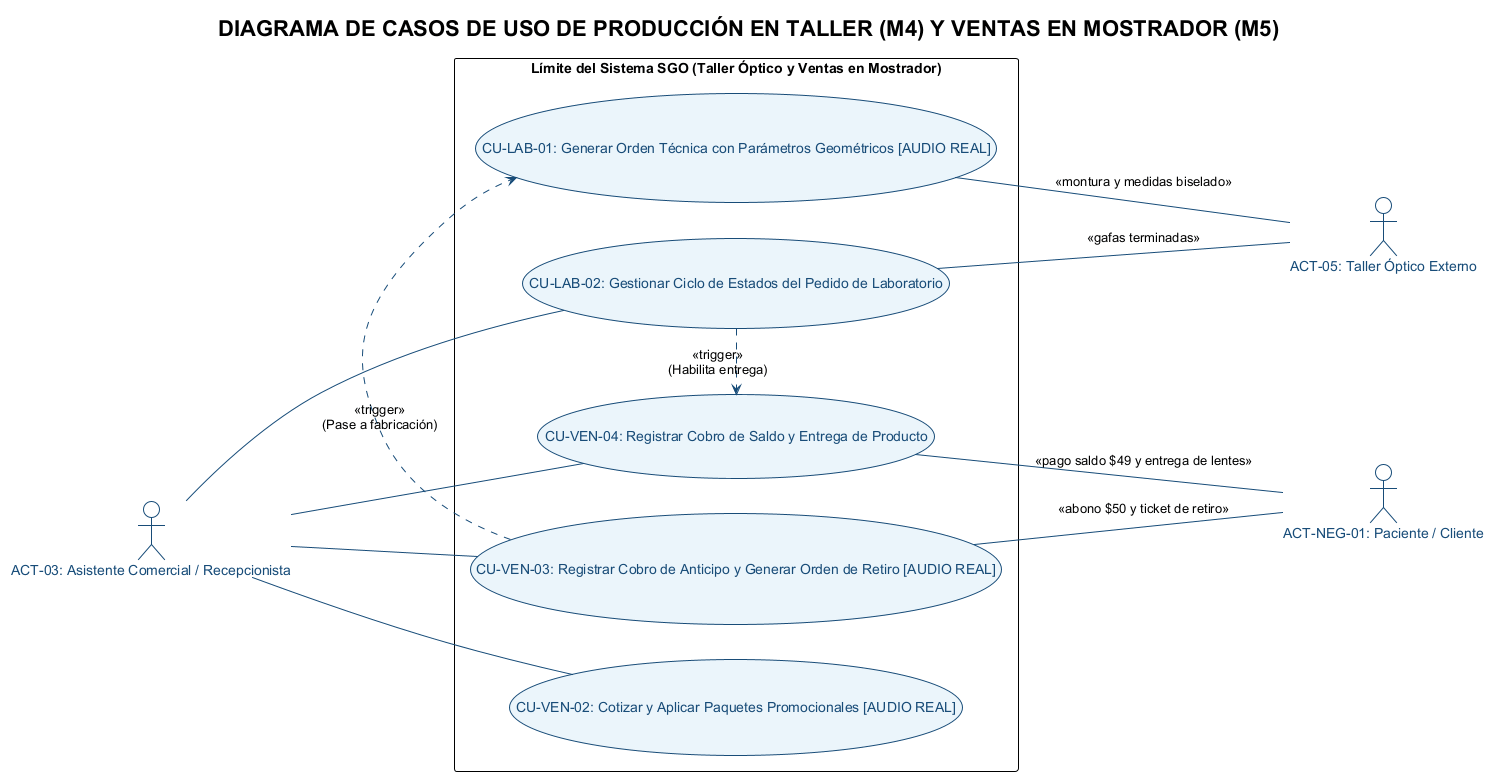
\includegraphics[width=0.90\textwidth]{pictures/diagrama_cu_taller_ventas.png}
    \caption{Diagrama de Casos de Uso de Producción en Taller (M4) y Ventas en Mostrador (M5).}
    \label{fig:diagrama_cu_taller_ventas}
\end{figure}

\begin{figure}[H]
    \centering
    % IMAGEN: Máquina de Estados del Pedido de Taller
    % Guardar como: pictures/maquina_estados_taller.png en Overleaf
    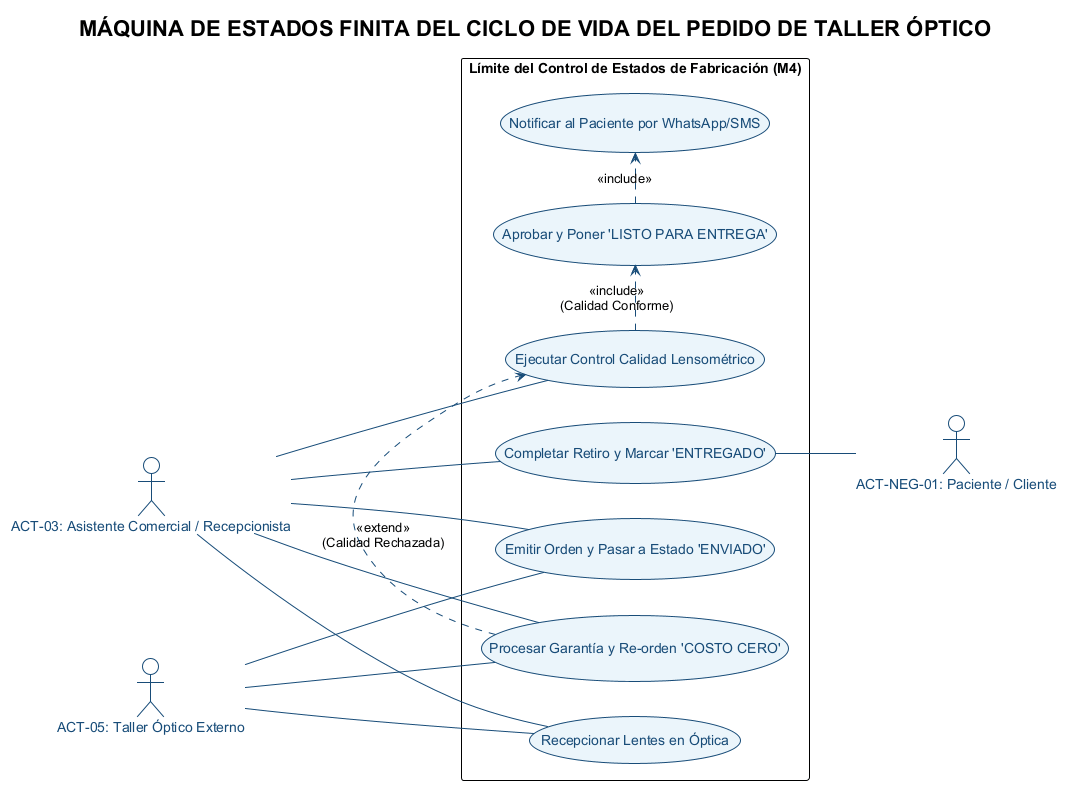
\includegraphics[width=0.82\textwidth]{pictures/maquina_estados_taller.png}
    \caption{Máquina de Estados Finita del Ciclo de Vida del Pedido de Taller Óptico.}
    \label{fig:maquina_estados_taller}
\end{figure}

\section{Diagrama de Casos de Uso: Facturación SRI (M6) e Inteligencia Artificial (M7)}
\begin{figure}[H]
    \centering
    % IMAGEN: Diagrama de Casos de Uso M6 y M7
    % Guardar como: pictures/diagrama_cu_sri_ia.png en Overleaf
    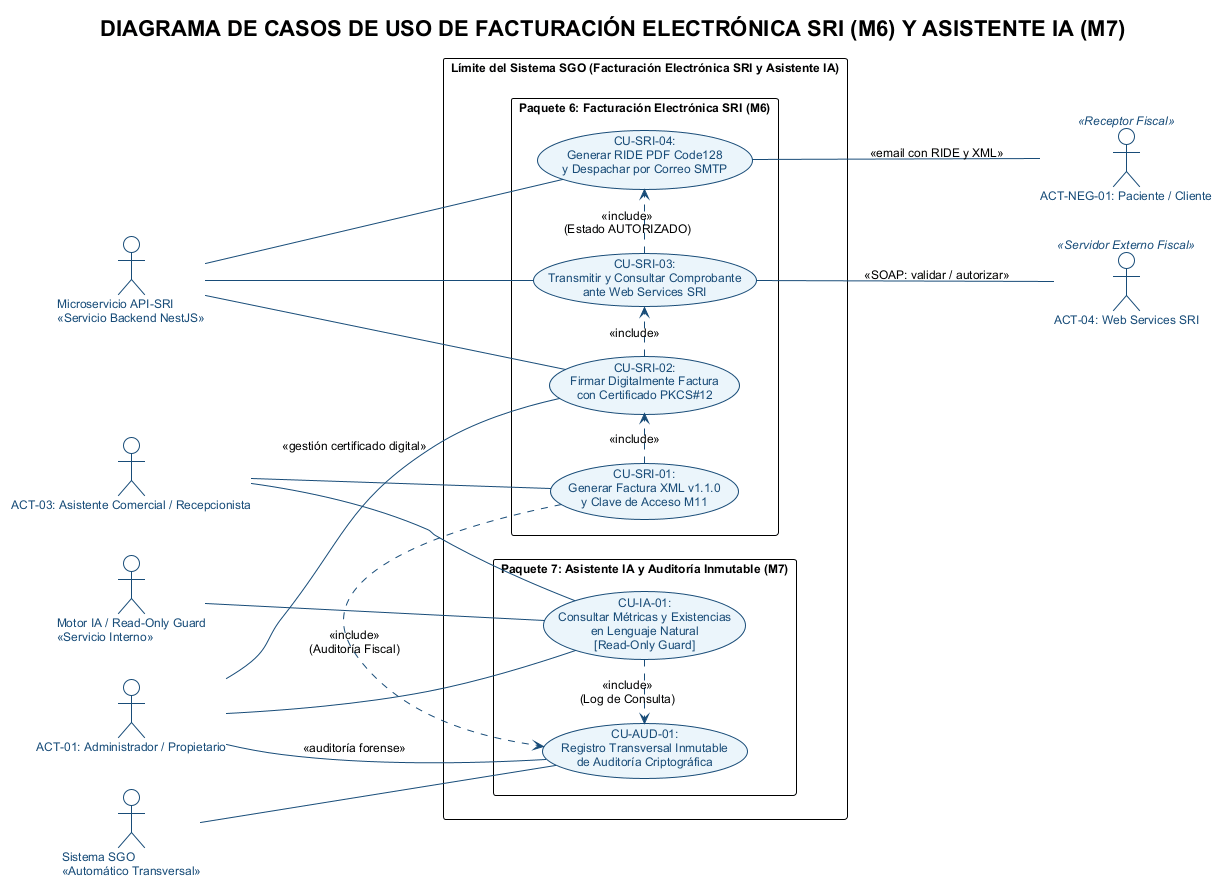
\includegraphics[width=0.90\textwidth]{pictures/diagrama_cu_sri_ia.png}
    \caption{Diagrama de Casos de Uso de Facturación Electrónica SRI (M6) y Asistente IA (M7).}
    \label{fig:diagrama_cu_sri_ia}
\end{figure}

\begin{figure}[H]
    \centering
    % IMAGEN: Arquitectura del Read-Only Guard
    % Guardar como: pictures/arquitectura_readonly_guard.png en Overleaf
    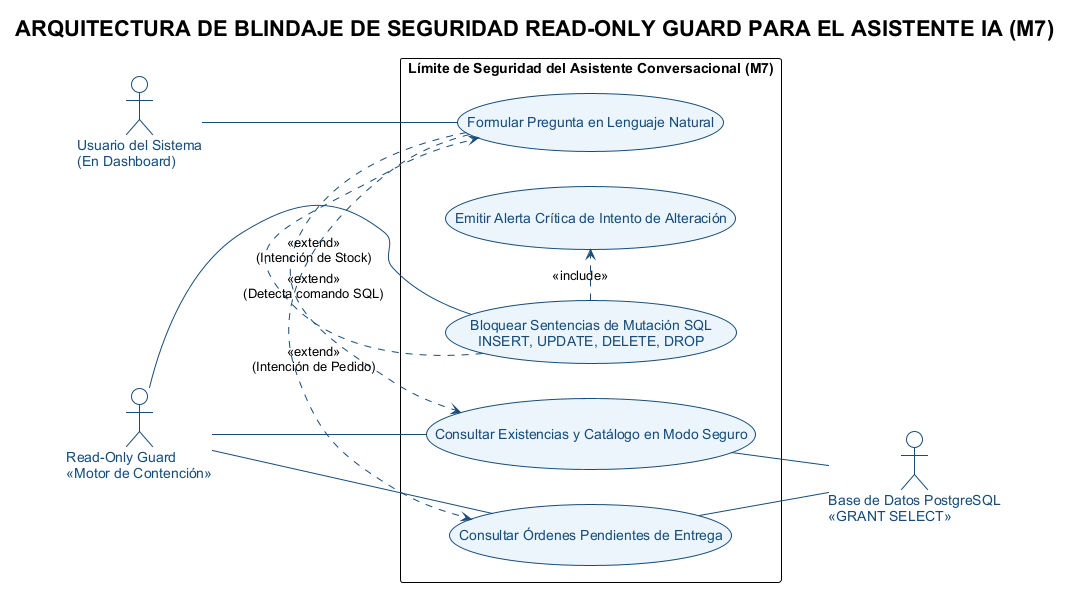
\includegraphics[width=0.85\textwidth]{pictures/arquitectura_readonly_guard.png}
    \caption{Arquitectura de Blindaje de Seguridad Read-Only Guard para el Asistente IA.}
    \label{fig:arquitectura_readonly_guard}
\end{figure}

% ==============================================================================
% CAPÍTULO 4: ESPECIFICACIÓN DETALLADA DE CASOS DE USO (FICHAS PMO)
% ==============================================================================
\newpage
\chapter{Especificación Detallada de los 23 Casos de Uso}

A continuación se presenta la especificación estructurada conforme a la plantilla oficial de PMOInformática:

% ------------------------------------------------------------------------------
% PAQUETE 1: SEGURIDAD (M1)
% ------------------------------------------------------------------------------
\section{Paquete 1: Gestión de Acceso y Seguridad RBAC (M1)}

\subsection{CU-SEG-01: Iniciar Sesión y Validar Credenciales RBAC}
\begin{table}[H]
\centering
\small
\begin{tabularx}{\textwidth}{|L{3.5cm}|X|}
\hline
\rowcolor{primaryBlue}\color{white}\textbf{Caso de Uso:} & \textbf{CU-SEG-01: Iniciar Sesión y Validar Credenciales RBAC} \\
\hline
\textbf{Actores:} & Usuario Autenticado (ACT-01 Administrador, ACT-02 Optometrista, ACT-03 Asistente). \\
\hline
\textbf{Tipo:} & Primario \\
\hline
\textbf{Referencias:} & SRS v2.0 (RF-01, RF-02) / Reglas: RN-SEG-01, RN-SEG-02 / S-Tags: S-TAG-AUTH-01. \\
\hline
\textbf{Precondición:} & Conectividad activa al backend; cuenta en estado 'ACTIVO'; terminal libre de sesión. \\
\hline
\textbf{Postcondición:} & Token JWT RS256 emitido (TTL 8h); evento en \texttt{audit\_logs}; redirección por rol. \\
\hline
\textbf{Descripción:} & Autentica al personal contrastando usuario y contraseña contra el hash Argon2id, generando la sesión criptográfica segura con perfil de navegación RBAC. \\
\hline
\end{tabularx}
\end{table}

\begin{table}[H]
\centering
\small
\begin{tabularx}{\textwidth}{|c|L{3.5cm}|X|}
\hline
\rowcolor{lightGray}\textbf{Paso} & \textbf{Ejecutor} & \textbf{Curso Normal (Flujo Básico)} \\
\hline
1 & Usuario Autenticado & Accede a la pantalla de autenticación del sistema SGO. \\
\hline
2 & Usuario Autenticado & Introduce su nombre de usuario y contraseña secreta. \\
\hline
3 & Usuario Autenticado & Pulsa el botón "Iniciar Sesión". \\
\hline
4 & Sistema SGO & Sanitiza campos y verifica existencia del usuario en la base de datos. \\
\hline
5 & Sistema SGO & Comprueba que \texttt{estado\_activo = TRUE} y que \texttt{intentos\_fallidos < 3}. \\
\hline
6 & Sistema SGO & [\texttt{<<include>>}] Verifica el hash mediante algoritmo criptográfico Argon2id. \\
\hline
7 & Sistema SGO & Restablece \texttt{intentos\_fallidos = 0} y actualiza \texttt{ultimo\_login} UTC. \\
\hline
8 & Sistema SGO & Genera token JWT RS256 y cookie HttpOnly con flag \texttt{SameSite=Strict}. \\
\hline
9 & Sistema SGO & [\texttt{<<include>>}] Inserta registro en \texttt{audit\_logs} con IP y user\_id. \\
\hline
10 & Sistema SGO & Redirige a vista autorizada (Admin: Métricas, Optom: Consulta, Asist: POS). \\
\hline
\end{tabularx}
\caption{Curso Normal de CU-SEG-01.}
\end{table}

\begin{table}[H]
\centering
\small
\begin{tabularx}{\textwidth}{|c|L{4.2cm}|X|}
\hline
\rowcolor{lightGray}\textbf{Ref.} & \textbf{Condición Detonante} & \textbf{Cursos Alternos (Excepciones y Variaciones)} \\
\hline
4a & Usuario no existe & Simula cómputo hash; muestra "Credenciales incorrectas"; log anónimo. \\
\hline
5a & Cuenta bloqueada ($\ge$ 3) & Deniega acceso sin evaluar clave: "Cuenta bloqueada por seguridad". \\
\hline
6a & Contraseña no coincide & Incrementa contador (+1). Si llega a 3, bloquea la cuenta (\texttt{estado=FALSE}). \\
\hline
\end{tabularx}
\caption{Cursos Alternos de CU-SEG-01.}
\end{table}

\subsection{CU-SEG-02: Cerrar Sesión por Inactividad o Petición}
\begin{table}[H]
\centering
\small
\begin{tabularx}{\textwidth}{|L{3.5cm}|X|}
\hline
\rowcolor{primaryBlue}\color{white}\textbf{Caso de Uso:} & \textbf{CU-SEG-02: Cerrar Sesión por Inactividad o Petición} \\
\hline
\textbf{Actores:} & Usuario Autenticado (ACT-01, ACT-02, ACT-03), Temporizador del Sistema. \\
\hline
\textbf{Tipo:} & Secundario / S-Tag: S-TAG-AUTH-02, S-TAG-ACC-02. \\
\hline
\textbf{Precondición:} & Sesión abierta con token JWT activo en la terminal. \\
\hline
\textbf{Postcondición:} & Token invalidado en lista negra (Redis Blacklist); caché purgada; retorno a login. \\
\hline
\textbf{Descripción:} & Finaliza la sesión por decisión voluntaria del operador o de forma forzada tras 15 minutos de inactividad, evitando accesos no autorizados a datos clínicos en terminales desatendidas. \\
\hline
\end{tabularx}
\end{table}

% ------------------------------------------------------------------------------
% PAQUETE 2: PACIENTES (M2)
% ------------------------------------------------------------------------------
\section{Paquete 2: Gestión Demográfica de Pacientes (M2)}

\subsection{CU-PAC-01: Registrar Paciente con Validación Módulo 10}
\begin{table}[H]
\centering
\small
\begin{tabularx}{\textwidth}{|L{3.5cm}|X|}
\hline
\rowcolor{primaryBlue}\color{white}\textbf{Caso de Uso:} & \textbf{CU-PAC-01: Registrar Paciente con Validación Módulo 10} \\
\hline
\textbf{Actores:} & Asistente Comercial (ACT-03), Optometrista Clínico (ACT-02). \\
\hline
\textbf{Tipo:} & Primario / Reglas: RN-PAC-01 (Módulo 10), RN-PAC-03 (Soft Delete). \\
\hline
\textbf{Precondición:} & Operador autenticado; paciente no registrado previamente en el sistema. \\
\hline
\textbf{Postcondición:} & Registro creado en \texttt{pacientes} con UUID único y cédula indexada de forma única. \\
\hline
\textbf{Descripción:} & Captura la filiación del paciente evaluando algorítmicamente en tiempo real la validez provincial y el dígito verificador de la cédula ecuatoriana mediante Módulo 10. \\
\hline
\end{tabularx}
\end{table}

\begin{table}[H]
\centering
\small
\begin{tabularx}{\textwidth}{|c|L{3.5cm}|X|}
\hline
\rowcolor{lightGray}\textbf{Paso} & \textbf{Ejecutor} & \textbf{Curso Normal (Flujo Básico)} \\
\hline
1 & Asistente Comercial & Accede al formulario "Nuevo Paciente" desde el menú de recepción. \\
\hline
2 & Asistente Comercial & Introduce la cédula de ciudadanía de 10 dígitos. \\
\hline
3 & Sistema SGO & [\texttt{<<include>>}] Ejecuta Módulo 10: verifica provincia (01-24 o 30), tercer dígito < 6 y calcula residuo ponderado de coeficientes (2,1,2,1...). \\
\hline
4 & Sistema SGO & Constata que la cédula no se encuentre duplicada en la base de datos. \\
\hline
5 & Asistente Comercial & Completa: nombres, apellidos, fecha nacimiento, celular, email, ocupación. \\
\hline
6 & Sistema SGO & Calcula la edad cronológica exacta y valida formato de contacto. \\
\hline
7 & Asistente Comercial & Pulsa "Guardar Paciente". \\
\hline
8 & Sistema SGO & Persiste registro (\texttt{soft\_delete=FALSE}) y emite log en \texttt{audit\_logs}. \\
\hline
\end{tabularx}
\caption{Curso Normal de CU-PAC-01.}
\end{table}

\subsection{CU-PAC-02: Registrar Menor de Edad sin Documento de Identidad}
\begin{table}[H]
\centering
\small
\begin{tabularx}{\textwidth}{|L{3.5cm}|X|}
\hline
\rowcolor{primaryBlue}\color{white}\textbf{Caso de Uso:} & \textbf{CU-PAC-02: Registrar Menor de Edad sin Documento de Identidad} \\
\hline
\textbf{Actores:} & Asistente Comercial (ACT-03), Optometrista Clínico (ACT-02). \\
\hline
\textbf{Tipo:} & Opcional / Extensión de CU-PAC-01 / Regla: RN-PAC-02. \\
\hline
\textbf{Descripción:} & Permite el registro de infantes no cedulados asignando una clave temporal sintética estructurada (\texttt{MEN-YYYYMMDD-XXXX}) vinculada indisolublemente al tutor legal verificado. \\
\hline
\end{tabularx}
\end{table}

\subsection{CU-PAC-03: Búsqueda Predictiva de Pacientes}
\begin{table}[H]
\centering
\small
\begin{tabularx}{\textwidth}{|L{3.5cm}|X|}
\hline
\rowcolor{primaryBlue}\color{white}\textbf{Caso de Uso:} & \textbf{CU-PAC-03: Búsqueda Predictiva de Pacientes} \\
\hline
\textbf{Actores:} & Usuario Autenticado (ACT-01, ACT-02, ACT-03). \\
\hline
\textbf{Tipo:} & Primario / Rendimiento: Tiempo de respuesta $< 200$ ms. \\
\hline
\textbf{Descripción:} & Localiza en tiempo real registros de pacientes al ingresar $\ge 3$ caracteres en la barra universal, mediante indexación trigram por cédula, nombres, apellidos o teléfono. \\
\hline
\end{tabularx}
\end{table}

% ------------------------------------------------------------------------------
% PAQUETE 3: CLÍNICO (M3)
% ------------------------------------------------------------------------------
\newpage
\section{Paquete 3: Atención Clínica y Refracción Integral (M3)}

\subsection{CU-CLI-01: Registrar Anamnesis y Motivo de Consulta}
\begin{table}[H]
\centering
\small
\begin{tabularx}{\textwidth}{|L{3.5cm}|X|}
\hline
\rowcolor{primaryBlue}\color{white}\textbf{Caso de Uso:} & \textbf{CU-CLI-01: Registrar Anamnesis y Motivo de Consulta} \\
\hline
\textbf{Actores:} & Optometrista Clínico (ACT-02). \\
\hline
\textbf{Tipo:} & Primario / SRS v2.0 (RF-13). \\
\hline
\textbf{Descripción:} & Documenta síntomas referidos (visión borrosa, astenopía, cefalea), factores ocupacionales en pantallas y antecedentes sistémicos u oftalmológicos familiares. \\
\hline
\end{tabularx}
\end{table}

\subsection{CU-CLI-02: Registrar Lensometría y Estado de Gafas Previas [AUDIO REAL]}
\begin{table}[H]
\centering
\small
\begin{tabularx}{\textwidth}{|L{3.5cm}|X|}
\hline
\rowcolor{primaryBlue}\color{white}\textbf{Caso de Uso:} & \textbf{CU-CLI-02: Registrar Lensometría y Estado de Gafas Previas} \\
\hline
\textbf{Actores:} & Optometrista Clínico (ACT-02). \\
\hline
\textbf{Tipo:} & Primario / Elicitado de Audio Clínico Real / Regla: RN-CLI-04. \\
\hline
\textbf{Precondición:} & Consulta abierta; gafas físicas del paciente disponibles en lensómetro. \\
\hline
\textbf{Postcondición:} & Fórmula dioptrica anterior y diagnóstico de daño guardados para comparación. \\
\hline
\textbf{Descripción:} & Captura la graduación in situ de los lentes en uso del paciente (+1.75 / -1.50 según audio), su material (plástico CR-39 con filtro azul) y registra el daño físico detectado (luna astillada en esquina inferior por falta de bisel protegido en armazón semialaire). \\
\hline
\end{tabularx}
\end{table}

\begin{table}[H]
\centering
\small
\begin{tabularx}{\textwidth}{|c|L{3.5cm}|X|}
\hline
\rowcolor{lightGray}\textbf{Paso} & \textbf{Ejecutor} & \textbf{Curso Normal (Flujo Básico)} \\
\hline
1 & Optometrista Clínico & Coloca las gafas previas en el lensómetro del consultorio. \\
\hline
2 & Optometrista Clínico & Accede a la pestaña "Lensometría / Lentes Previos". \\
\hline
3 & Optometrista Clínico & Ingresa graduación OD: Esfera +1.75 D, Cilindro -1.50 D, Eje 10°. \\
\hline
4 & Optometrista Clínico & Ingresa graduación OI: Esfera +1.75 D, Cilindro -1.50 D, Eje 175°. \\
\hline
5 & Optometrista Clínico & Selecciona material (Plástico CR-39) y filtro detectado (Filtro Azul). \\
\hline
6 & Optometrista Clínico & Documenta daño estructural: "Luna astillada en esquina inferior por armazón semialaire". \\
\hline
7 & Sistema SGO & Persiste registro en \texttt{lensometria\_previa} y carga comparativa dioptrica. \\
\hline
\end{tabularx}
\caption{Curso Normal de CU-CLI-02.}
\end{table}

\subsection{CU-CLI-03: Registrar Pruebas Objetivas y Queratometría [AUDIO REAL]}
\begin{table}[H]
\centering
\small
\begin{tabularx}{\textwidth}{|L{3.5cm}|X|}
\hline
\rowcolor{primaryBlue}\color{white}\textbf{Caso de Uso:} & \textbf{CU-CLI-03: Registrar Pruebas Objetivas y Queratometría} \\
\hline
\textbf{Actores:} & Optometrista Clínico (ACT-02). \\
\hline
\textbf{Tipo:} & Primario / Elicitado de Audio Clínico Real / Regla: RN-CLI-05. \\
\hline
\textbf{Descripción:} & Registra las lecturas corneales K1/K2 y autorrefractometría computarizada, calculando automáticamente el astigmatismo corneal ($\Delta K = K_2 - K_1$) y precargando el foróptero. \\
\hline
\end{tabularx}
\end{table}

\subsection{CU-CLI-04: Examen Refractivo y Confort Ambulatorio en Marcha [AUDIO REAL]}
\begin{table}[H]
\centering
\small
\begin{tabularx}{\textwidth}{|L{3.5cm}|X|}
\hline
\rowcolor{primaryBlue}\color{white}\textbf{Caso de Uso:} & \textbf{CU-CLI-04: Examen Refractivo y Confort Ambulatorio en Marcha} \\
\hline
\textbf{Actores:} & Optometrista Clínico (ACT-02), Paciente / Cliente (ACT-NEG-01). \\
\hline
\textbf{Tipo:} & Primario / Elicitado de Audio / Reglas: RN-CLI-01, RN-CLI-02, RN-CLI-03. \\
\hline
\textbf{Precondición:} & Consulta clínica activa; pruebas objetivas y lensometría completadas. \\
\hline
\textbf{Postcondición:} & Refracción definitiva sellada inmutablemente con hash SHA-256; marcha aprobada. \\
\hline
\textbf{Descripción:} & Determina la corrección subjetiva con foróptero y cartilla Snellen. Exige mandatoriamente montar los lentes en montura de prueba y realizar el test de marcha en piso para constatar confort visual y ausencia de mareos antes de sellar la prescripción. \\
\hline
\end{tabularx}
\end{table}

\begin{table}[H]
\centering
\small
\begin{tabularx}{\textwidth}{|c|L{3.5cm}|X|}
\hline
\rowcolor{lightGray}\textbf{Paso} & \textbf{Ejecutor} & \textbf{Curso Normal (Flujo Básico)} \\
\hline
1 & Optometrista Clínico & Registra agudeza visual sin corrección (OD: 20/70, OI: 20/80). \\
\hline
2 & Optometrista Clínico & Gradúa con foróptero en pasos de 0.25 D (OD: +2.00/-1.75x10°, OI: +2.00/-1.75x175°). \\
\hline
3 & Sistema SGO & [\texttt{<<include>>}] Valida cilindro negativo y muestra comparativa con lente previa. \\
\hline
4 & Optometrista Clínico & Monta la graduación en la armazón de prueba ambulatoria. \\
\hline
5 & Paciente & Camina por el consultorio observando el piso, muebles y vitrinas. \\
\hline
6 & Paciente & Confirma confort pleno ("piso plano, nítido y sin mareo"). \\
\hline
7 & Optometrista Clínico & Marca checkbox obligatorio: "[x] Confort ambulatorio verificado sin mareo". \\
\hline
8 & Optometrista Clínico & Registra Distancia Nasopupilar monocular (OD: 31.5 mm, OI: 32.0 mm). \\
\hline
9 & Sistema SGO & Sella la refracción en PostgreSQL con firma inmutable SHA-256. \\
\hline
\end{tabularx}
\caption{Curso Normal de CU-CLI-04.}
\end{table}

\subsection{CU-CLI-05: Emitir Receta Óptica Digital y Certificado Visual}
\begin{table}[H]
\centering
\small
\begin{tabularx}{\textwidth}{|L{3.5cm}|X|}
\hline
\rowcolor{primaryBlue}\color{white}\textbf{Caso de Uso:} & \textbf{CU-CLI-05: Emitir Receta Óptica Digital y Certificado Visual} \\
\hline
\textbf{Actores:} & Optometrista Clínico (ACT-02), Paciente / Cliente (ACT-NEG-01). \\
\hline
\textbf{Tipo:} & Primario / SRS v2.0 (RF-14, RF-15) / S-Tag: S-TAG-AUTH-03. \\
\hline
\textbf{Descripción:} & Genera la receta médica con membrete institucional de Óptica de Estudio, código QR de verificación de autenticidad, diagnóstico CIE-10 (H52.2 Astigmatismo) y firma profesional. \\
\hline
\end{tabularx}
\end{table}

\begin{figure}[H]
    \centering
    % IMAGEN: Formato de Receta Médica Emitida por el SGO con Código QR
    % Guardar como: pictures/muestra_receta_optica_qr.png en Overleaf
    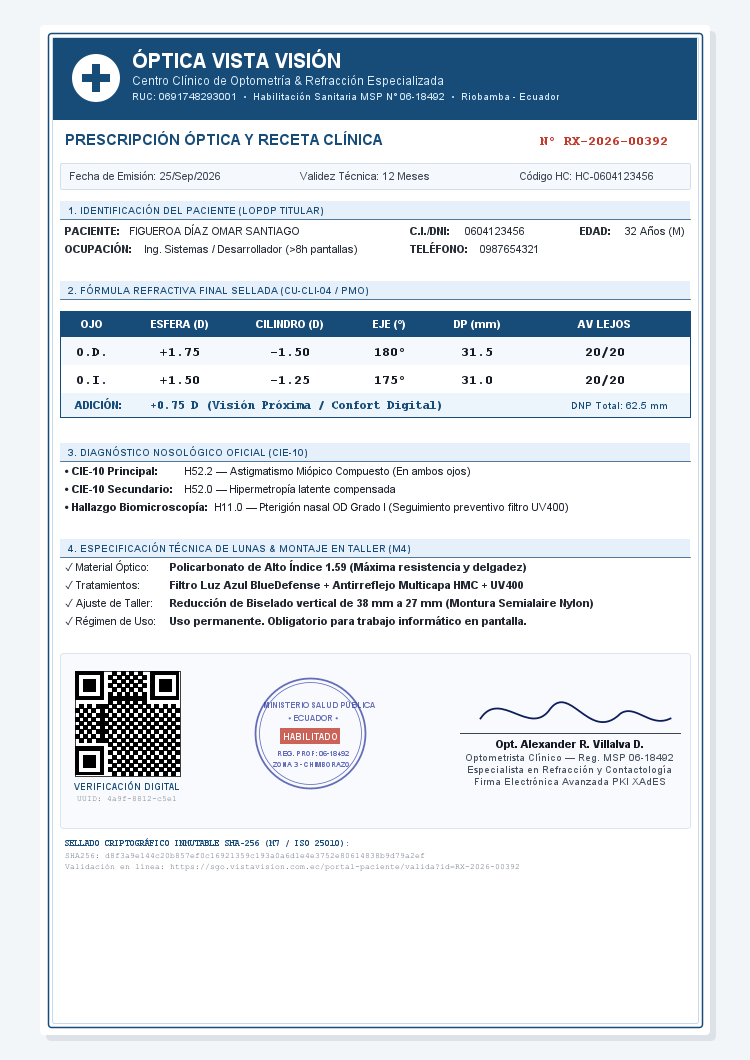
\includegraphics[width=0.75\textwidth]{pictures/muestra_receta_optica_qr.png}
    \caption{Ejemplo de Prescripción Óptica Digital con Código QR y Sello MSP (CU-CLI-05).}
    \label{fig:muestra_receta_optica_qr}
\end{figure}

\subsection{CU-CLI-06: Evaluación de Polo Anterior y Seguimiento Patológico [AUDIO REAL]}
\begin{table}[H]
\centering
\small
\begin{tabularx}{\textwidth}{|L{3.5cm}|X|}
\hline
\rowcolor{primaryBlue}\color{white}\textbf{Caso de Uso:} & \textbf{CU-CLI-06: Evaluación de Polo Anterior y Seguimiento Patológico} \\
\hline
\textbf{Actores:} & Optometrista Clínico (ACT-02), Paciente / Cliente (ACT-NEG-01). \\
\hline
\textbf{Tipo:} & Secundario / Elicitado de Audio / Regla: RN-CLI-06. \\
\hline
\textbf{Descripción:} & Documenta el hallazgo biomicroscópico de pterigión en cara interna nasal (Grado I, sin invasión corneal), estampando en la receta advertencias preventivas mandatorias (uso obligatorio de filtro solar UV400 y prohibición de frotamiento ocular). \\
\hline
\end{tabularx}
\end{table}

% ------------------------------------------------------------------------------
% PAQUETE 4: TALLER (M4)
% ------------------------------------------------------------------------------
\newpage
\section{Paquete 4: Taller y Laboratorio Óptico (M4)}

\subsection{CU-LAB-01: Generar Orden Técnica de Taller con Parámetros Geométricos [AUDIO REAL]}
\begin{table}[H]
\centering
\small
\begin{tabularx}{\textwidth}{|L{3.5cm}|X|}
\hline
\rowcolor{primaryBlue}\color{white}\textbf{Caso de Uso:} & \textbf{CU-LAB-01: Generar Orden Técnica con Parámetros Geométricos} \\
\hline
\textbf{Actores:} & Optometrista Clínico (ACT-02), Asistente Comercial (ACT-03). \\
\hline
\textbf{Tipo:} & Primario / Elicitado de Audio / Reglas: RN-LAB-01, RN-LAB-02. \\
\hline
\textbf{Precondición:} & Refracción concluida; armazón y material de lunas seleccionados. \\
\hline
\textbf{Postcondición:} & Orden creada en estado 'PENDIENTE' con datos médicos disociados (LOPDP). \\
\hline
\textbf{Descripción:} & Construye la ficha técnica para el laboratorio suprimiendo datos patológicos. Especifica parámetros milimétricos de biselado para armazón semialaire (nylon): altura original de montura de 38 mm con reducción vertical a 27 mm para luna biselada. \\
\hline
\end{tabularx}
\end{table}

\begin{table}[H]
\centering
\small
\begin{tabularx}{\textwidth}{|c|L{3.5cm}|X|}
\hline
\rowcolor{lightGray}\textbf{Paso} & \textbf{Ejecutor} & \textbf{Curso Normal (Flujo Básico)} \\
\hline
1 & Optometrista / Asist. & Selecciona prescripción y pulsa "Generar Orden de Taller". \\
\hline
2 & Sistema SGO & [\texttt{<<include>>}] Disocia datos médicos (elimina CIE-10 y notas clínicas). \\
\hline
3 & Optometrista / Asist. & Selecciona montura semialaire metálica y material policarbonato filtro azul. \\
\hline
4 & Optometrista / Asist. & Ingresa DNP (31.5/32.0 mm) y alturas focales pupilares (18/18 mm). \\
\hline
5 & Optometrista / Asist. & Especifica cotas de biselado: Altura original 38 mm $\to$ Altura luna 27 mm. \\
\hline
6 & Sistema SGO & Valida que 27 mm aloje la altura focal y emite la orden técnica de corte. \\
\hline
\end{tabularx}
\caption{Curso Normal de CU-LAB-01.}
\end{table}

\subsection{CU-LAB-02: Gestionar Ciclo de Estados del Pedido de Laboratorio}
\begin{table}[H]
\centering
\small
\begin{tabularx}{\textwidth}{|L{3.5cm}|X|}
\hline
\rowcolor{primaryBlue}\color{white}\textbf{Caso de Uso:} & \textbf{CU-LAB-02: Gestionar Ciclo de Estados del Pedido} \\
\hline
\textbf{Actores:} & Asistente Comercial (ACT-03), Taller Óptico Externo (ACT-05). \\
\hline
\textbf{Tipo:} & Secundario / Control de Máquina de Estados. \\
\hline
\textbf{Descripción:} & Controla las transiciones del encargo: \texttt{ENVIADO\_A\_TALLER} $\to$ \texttt{RECIBIDO\_EN\_OPTICA} $\to$ \texttt{CONTROL\_CALIDAD\_OK} (con lensómetro) $\to$ \texttt{LISTO\_PARA\_ENTREGA} con notificación automática al cliente. \\
\hline
\end{tabularx}
\end{table}

\subsection{CU-LAB-03: Registrar Incidencia o Garantía Técnica}
\begin{table}[H]
\centering
\small
\begin{tabularx}{\textwidth}{|L{3.5cm}|X|}
\hline
\rowcolor{primaryBlue}\color{white}\textbf{Caso de Uso:} & \textbf{CU-LAB-03: Registrar Incidencia o Garantía Técnica} \\
\hline
\textbf{Actores:} & Asistente Comercial (ACT-03), Optometrista Clínico (ACT-02). \\
\hline
\textbf{Tipo:} & Opcional / Gestión de Garantías a Costo Cero. \\
\hline
\textbf{Descripción:} & Documenta no-conformidades físicas (lunas rayadas, aberraciones de bisel) y emite re-orden de producción vinculada sin costo adicional al cliente. \\
\hline
\end{tabularx}
\end{table}

% ------------------------------------------------------------------------------
% PAQUETE 5: VENTAS Y CAJA (M5)
% ------------------------------------------------------------------------------
\newpage
\section{Paquete 5: Ventas, Caja y Mostrador (M5)}

\subsection{CU-VEN-01: Registrar Venta con Descuento Híbrido de Inventario}
\begin{table}[H]
\centering
\small
\begin{tabularx}{\textwidth}{|L{3.5cm}|X|}
\hline
\rowcolor{primaryBlue}\color{white}\textbf{Caso de Uso:} & \textbf{CU-VEN-01: Registrar Venta con Descuento Híbrido de Inventario} \\
\hline
\textbf{Actores:} & Asistente Comercial (ACT-03). \\
\hline
\textbf{Tipo:} & Primario / SRS v2.0 (RF-20, RF-21) / Regla: RN-VEN-01. \\
\hline
\textbf{Descripción:} & Comercializa accesorios o productos terminados con decremento atómico del stock físico en PostgreSQL y registro de cobro en caja. \\
\hline
\end{tabularx}
\end{table}

\subsection{CU-VEN-02: Cotizar y Aplicar Paquetes Promocionales [AUDIO REAL]}
\begin{table}[H]
\centering
\small
\begin{tabularx}{\textwidth}{|L{3.5cm}|X|}
\hline
\rowcolor{primaryBlue}\color{white}\textbf{Caso de Uso:} & \textbf{CU-VEN-02: Cotizar y Aplicar Paquetes Promocionales} \\
\hline
\textbf{Actores:} & Asistente Comercial (ACT-03), Optometrista Clínico (ACT-02). \\
\hline
\textbf{Tipo:} & Primario / Elicitado de Audio / Regla: RN-VEN-02. \\
\hline
\textbf{Descripción:} & Aplica combos promocionales (Armazón semialaire + Lunas policarbonato filtro azul por tarifa plana de $99.00 USD frente a tarifa regular de $135.00 USD), desglosando ponderadamente los costos para control de inventario. \\
\hline
\end{tabularx}
\end{table}

\subsection{CU-VEN-03: Registrar Cobro de Anticipo y Generar Orden de Retiro [AUDIO REAL]}
\begin{table}[H]
\centering
\small
\begin{tabularx}{\textwidth}{|L{3.5cm}|X|}
\hline
\rowcolor{primaryBlue}\color{white}\textbf{Caso de Uso:} & \textbf{CU-VEN-03: Registrar Cobro de Anticipo y Orden de Retiro} \\
\hline
\textbf{Actores:} & Asistente Comercial (ACT-03), Paciente / Cliente (ACT-NEG-01). \\
\hline
\textbf{Tipo:} & Primario / Elicitado de Audio / Regla: RN-VEN-03. \\
\hline
\textbf{Precondición:} & Cotización de combo aprobada; orden técnica de taller enlazada. \\
\hline
\textbf{Postcondición:} & Cobro de abono registrado; saldo remanente fijado; ticket térmico impreso. \\
\hline
\textbf{Descripción:} & Cobra el anticipo monetario inicial ($50.00 USD en efectivo o transferencia), actualiza el pedido a 'ENVIADO\_A\_TALLER', calcula fecha de entrega en 2 días laborables (viernes) e imprime en ticketera de 80 mm la Orden de Retiro física con saldo pendiente de $49.00 USD. \\
\hline
\end{tabularx}
\end{table}

\begin{figure}[H]
    \centering
    % IMAGEN: Muestra de Ticket Térmico de Orden de Retiro (80 mm)
    % Guardar como: pictures/muestra_ticket_orden_retiro.png en Overleaf
    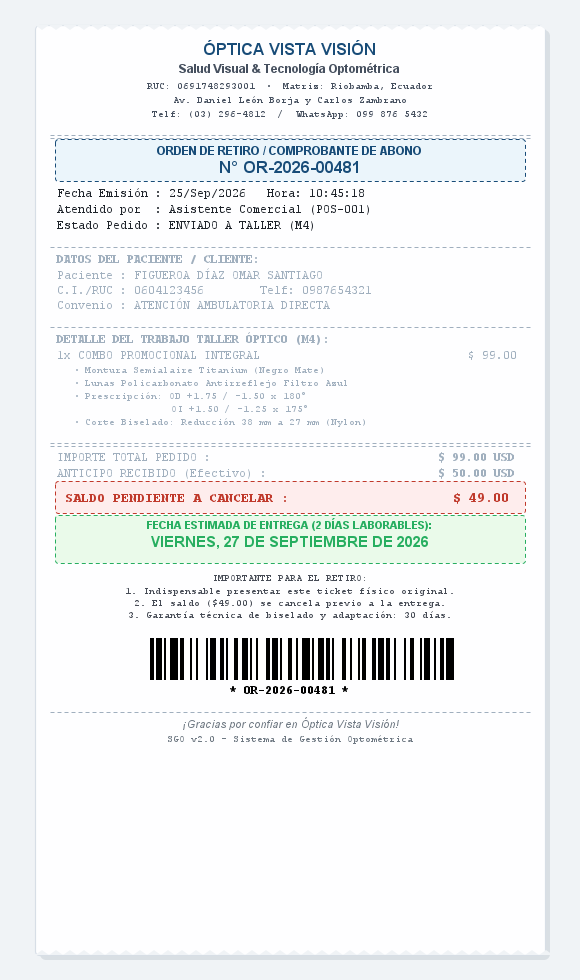
\includegraphics[width=0.60\textwidth]{pictures/muestra_ticket_orden_retiro.png}
    \caption{Ticket Térmico de 80 mm: Orden de Retiro con Desglose de Anticipo y Saldo (CU-VEN-03).}
    \label{fig:muestra_ticket_orden_retiro}
\end{figure}

\subsection{CU-VEN-04: Registrar Cobro de Saldo y Entrega de Producto}
\begin{table}[H]
\centering
\small
\begin{tabularx}{\textwidth}{|L{3.5cm}|X|}
\hline
\rowcolor{primaryBlue}\color{white}\textbf{Caso de Uso:} & \textbf{CU-VEN-04: Registrar Cobro de Saldo y Entrega de Producto} \\
\hline
\textbf{Actores:} & Asistente Comercial (ACT-03), Paciente / Cliente (ACT-NEG-01). \\
\hline
\textbf{Tipo:} & Primario / Liquidación Final de Trabajo Óptico. \\
\hline
\textbf{Descripción:} & Lee con pistola óptica el código de barras de la Orden de Retiro presentada por el cliente, recauda el saldo pendiente de $49.00 USD, transiciona el estado a 'ENTREGADO\_AL\_CLIENTE' y entrega los anteojos en su estuche. \\
\hline
\end{tabularx}
\end{table}

\subsection{CU-VEN-05: Realizar Cierre Diario y Arqueo Consolidado de Caja}
\begin{table}[H]
\centering
\small
\begin{tabularx}{\textwidth}{|L{3.5cm}|X|}
\hline
\rowcolor{primaryBlue}\color{white}\textbf{Caso de Uso:} & \textbf{CU-VEN-05: Realizar Cierre Diario y Arqueo Consolidado de Caja} \\
\hline
\textbf{Actores:} & Administrador / Propietario (ACT-01), Asistente Comercial (ACT-03). \\
\hline
\textbf{Tipo:} & Primario / Regla: RN-VEN-05 (Arqueo Ciego). \\
\hline
\textbf{Descripción:} & Realiza el balance financiero diario contrastando el efectivo físico contado a ciegas por el cajero contra los registros del sistema (ventas, anticipos y saldos), emitiendo la sábana consolidada. \\
\hline
\end{tabularx}
\end{table}

\subsection{CU-VEN-06: Anular Venta con Reversión Atómica ACID}
\begin{table}[H]
\centering
\small
\begin{tabularx}{\textwidth}{|L{3.5cm}|X|}
\hline
\rowcolor{primaryBlue}\color{white}\textbf{Caso de Uso:} & \textbf{CU-VEN-06: Anular Venta con Reversión Atómica ACID} \\
\hline
\textbf{Actores:} & Administrador / Propietario (ACT-01). \\
\hline
\textbf{Tipo:} & Secundario / Regla: RN-VEN-04 (Exclusividad del Administrador). \\
\hline
\textbf{Descripción:} & Revierte atómicamente una transacción en PostgreSQL (\texttt{BEGIN...COMMIT}): restituye el stock al inventario, inserta contra-asiento de egreso en caja y cancela la orden de taller en simultáneo. \\
\hline
\end{tabularx}
\end{table}

% ------------------------------------------------------------------------------
% PAQUETE 6: SRI (M6)
% ------------------------------------------------------------------------------
\newpage
\section{Paquete 6: Facturación Electrónica SRI (M6)}

\subsection{CU-SRI-01: Generar Factura XML v1.1.0 y Clave de Acceso M11}
\begin{table}[H]
\centering
\small
\begin{tabularx}{\textwidth}{|L{3.5cm}|X|}
\hline
\rowcolor{primaryBlue}\color{white}\textbf{Caso de Uso:} & \textbf{CU-SRI-01: Generar Factura XML v1.1.0 y Clave Módulo 11} \\
\hline
\textbf{Actores:} & Asistente Comercial (ACT-03), Microservicio API-SRI. \\
\hline
\textbf{Tipo:} & Primario / Ficha Técnica SRI v1.1.0 / Reglas: RN-SRI-01, RN-SRI-03. \\
\hline
\textbf{Descripción:} & Estructura el XML conforme al esquema XSD v1.1.0, calcula los 49 dígitos de la Clave de Acceso ponderada por Módulo 11 y bloquea emisiones a Consumidor Final superiores a $50.00 USD. \\
\hline
\end{tabularx}
\end{table}

\subsection{CU-SRI-02: Firmar Digitalmente Factura con Certificado PKCS\#12 (XAdES-BES)}
\begin{table}[H]
\centering
\small
\begin{tabularx}{\textwidth}{|L{3.5cm}|X|}
\hline
\rowcolor{primaryBlue}\color{white}\textbf{Caso de Uso:} & \textbf{CU-SRI-02: Firmar Factura con Certificado PKCS\#12 (XAdES-BES)} \\
\hline
\textbf{Actores:} & Microservicio API-SRI (NestJS), Administrador (ACT-01). \\
\hline
\textbf{Tipo:} & Primario / Criptografía y Firma Electrónica Avanzada. \\
\hline
\textbf{Descripción:} & Aplica firma enveloped XAdES-BES utilizando la llave privada RSA del archivo \texttt{.p12} custodiado en memoria, realizando canonicalización C14N y digest SHA-1 no repudiable. \\
\hline
\end{tabularx}
\end{table}

\subsection{CU-SRI-03: Transmitir y Consultar Comprobante ante Web Services SRI}
\begin{table}[H]
\centering
\small
\begin{tabularx}{\textwidth}{|L{3.5cm}|X|}
\hline
\rowcolor{primaryBlue}\color{white}\textbf{Caso de Uso:} & \textbf{CU-SRI-03: Transmitir y Consultar Comprobante ante SRI} \\
\hline
\textbf{Actores:} & Microservicio API-SRI, Web Services SRI (ACT-04). \\
\hline
\textbf{Tipo:} & Primario / SOAP Fuera de Línea / Regla: RN-SRI-02 (Contingencia). \\
\hline
\textbf{Descripción:} & Consume los métodos SOAP \texttt{validarComprobante} y \texttt{autorizacionComprobante}. Ante caídas de enlace o intermitencias del SRI, coloca el comprobante en cola de contingencia asíncrona sin bloquear la atención local en mostrador. \\
\hline
\end{tabularx}
\end{table}

\subsection{CU-SRI-04: Generar RIDE PDF Code128 y Despachar por Correo SMTP}
\begin{table}[H]
\centering
\small
\begin{tabularx}{\textwidth}{|L{3.5cm}|X|}
\hline
\rowcolor{primaryBlue}\color{white}\textbf{Caso de Uso:} & \textbf{CU-SRI-04: Generar RIDE PDF Code128 y Despachar por Correo SMTP} \\
\hline
\textbf{Actores:} & Microservicio API-SRI, Asistente Comercial (ACT-03), Paciente (ACT-NEG-01). \\
\hline
\textbf{Tipo:} & Secundario / Despacho Tributario Legal. \\
\hline
\textbf{Descripción:} & Compila el documento PDF oficial del RIDE en 300 DPI con código de barras lineal Code128 de los 49 dígitos y despacha correo SMTP al paciente con el PDF y XML autorizados adjuntos. \\
\hline
\end{tabularx}
\end{table}

\begin{figure}[H]
    \centering
    % IMAGEN: Muestra de RIDE PDF Oficial de Factura Electrónica SRI
    % Guardar como: pictures/muestra_ride_factura_sri.png en Overleaf
    \includegraphics[width=0.85\textwidth]{pictures/muestra_ride_factura_sri.png}
    \caption{Representación Impresa del Documento Electrónico (RIDE) con Código de Barras Code128.}
    \label{fig:muestra_ride_factura_sri}
\end{figure}

% ------------------------------------------------------------------------------
% PAQUETE 7: IA Y AUDITORÍA (M7)
% ------------------------------------------------------------------------------
\newpage
\section{Paquete 7: Asistente IA y Auditoría Inmutable (M7)}

\subsection{CU-IA-01: Consultar Métricas y Existencias en Lenguaje Natural (Read-Only Guard)}
\begin{table}[H]
\centering
\small
\begin{tabularx}{\textwidth}{|L{3.5cm}|X|}
\hline
\rowcolor{primaryBlue}\color{white}\textbf{Caso de Uso:} & \textbf{CU-IA-01: Consultar Métricas en Lenguaje Natural (Read-Only Guard)} \\
\hline
\textbf{Actores:} & Usuario Autenticado (ACT-00), Motor IA / Enrutador Léxico. \\
\hline
\textbf{Tipo:} & Secundario / Reglas: RN-IA-01 (Read-Only), RN-IA-02 (RBAC Guard). \\
\hline
\textbf{Descripción:} & Procesa preguntas en lenguaje natural sobre stock o estado de pedidos en el dashboard. Opera conectado a una sesión PostgreSQL exclusiva con permiso \texttt{GRANT SELECT}, bloqueando de raíz cualquier intento de modificación de datos. \\
\hline
\end{tabularx}
\end{table}

\subsection{CU-AUD-01: Registro Transversal Inmutable de Auditoría Criptográfica}
\begin{table}[H]
\centering
\small
\begin{tabularx}{\textwidth}{|L{3.5cm}|X|}
\hline
\rowcolor{primaryBlue}\color{white}\textbf{Caso de Uso:} & \textbf{CU-AUD-01: Registro Transversal Inmutable de Auditoría} \\
\hline
\textbf{Actores:} & Sistema SGO (Automático Transversal), Administrador (ACT-01). \\
\hline
\textbf{Tipo:} & Primario / Seguridad y No Repudio / S-Tag: S-TAG-ACC-08. \\
\hline
\textbf{Descripción:} & Intercepta cada evento sensible del software e inserta un asiento en \texttt{audit\_logs} encadenado criptográficamente mediante Hash Chain ($Hash_n = \text{SHA-256}(Hash_{n-1} + Registro_n)$), garantizando que las bitácoras sean de solo inserción (Append-Only). \\
\hline
\end{tabularx}
\end{table}

% ==============================================================================
% CAPÍTULO 5: MATRIZ DE TRAZABILIDAD Y PRUEBAS UAT
% ==============================================================================
\newpage
\chapter{Matriz de Trazabilidad Integral y Pruebas UAT}

\section{Matriz de Trazabilidad Bidireccional Completa}
La Tabla \ref{tab:matriz_trazabilidad} evidencia la correspondencia unívoca entre requisitos contractuales (SRS v2.0), hallazgos de campo del audio médico, casos de uso del sistema SGO y casos de prueba funcionales:

\begin{table}[H]
\centering
\scriptsize
\begin{tabularx}{\textwidth}{|L{2.2cm}|L{3.2cm}|L{2.3cm}|c|L{2.3cm}|L{2.5cm}|}
\hline
\rowcolor{primaryBlue}\color{white}\textbf{Origen} & \rowcolor{primaryBlue}\color{white}\textbf{Requisito / Audio} & \rowcolor{primaryBlue}\color{white}\textbf{Caso de Uso} & \rowcolor{primaryBlue}\color{white}\textbf{Mód.} & \rowcolor{primaryBlue}\color{white}\textbf{Seguridad ISO} & \rowcolor{primaryBlue}\color{white}\textbf{Caso Prueba UAT} \\
\hline
SRS v2.0 & RF-01: Login y RBAC & CU-SEG-01 & M1 & S-TAG-AUTH-01 & CP-UAT-SEG-01 \\
\hline
SRS v2.0 & RF-02: Cierre Sesión & CU-SEG-02 & M1 & S-TAG-AUTH-02 & CP-UAT-SEG-02 \\
\hline
SRS v2.0 & RF-03: Cédula Módulo 10 & CU-PAC-01 & M2 & S-TAG-INT-01 & CP-UAT-PAC-01 \\
\hline
SRS v2.0 & RF-04: Menores sin Cédula & CU-PAC-02 & M2 & S-TAG-INT-02 & CP-UAT-PAC-02 \\
\hline
SRS v2.0 & RF-05: Búsqueda Predictiva & CU-PAC-03 & M2 & S-TAG-INT-03 & CP-UAT-PAC-03 \\
\hline
SRS v2.0 & RF-13: Anamnesis / CIE-10 & CU-CLI-01 & M3 & S-TAG-INT-04 & CP-UAT-CLI-01 \\
\hline
\rowcolor{lightGray}\textbf{Audio Real} & \textbf{Lensometría / Daño Previo} & \textbf{CU-CLI-02} & \textbf{M3} & \textbf{S-TAG-INT-04} & \textbf{CP-UAT-CLI-02} \\
\hline
\rowcolor{lightGray}\textbf{Audio Real} & \textbf{Queratometría K1/K2} & \textbf{CU-CLI-03} & \textbf{M3} & \textbf{S-TAG-INT-04} & \textbf{CP-UAT-CLI-03} \\
\hline
\rowcolor{lightGray}\textbf{Audio Real} & \textbf{Test Marcha sin Mareo} & \textbf{CU-CLI-04} & \textbf{M3} & \textbf{S-TAG-INT-04} & \textbf{CP-UAT-CLI-04} \\
\hline
SRS v2.0 & RF-07 a 12: Refracción & CU-CLI-04 & M3 & S-TAG-INT-04 & CP-UAT-CLI-05 \\
\hline
SRS v2.0 & RF-14, 15: Receta Óptica & CU-CLI-05 & M3 & S-TAG-AUTH-03 & CP-UAT-CLI-06 \\
\hline
\rowcolor{lightGray}\textbf{Audio Real} & \textbf{Pterigión y Filtro UV400} & \textbf{CU-CLI-06} & \textbf{M3} & \textbf{S-TAG-INT-04} & \textbf{CP-UAT-CLI-07} \\
\hline
\rowcolor{lightGray}\textbf{Audio Real} & \textbf{Biselado 38 a 27 mm} & \textbf{CU-LAB-01} & \textbf{M4} & \textbf{S-TAG-CONF-03} & \textbf{CP-UAT-LAB-01} \\
\hline
SRS v2.0 & RF-10, 11, 16: Taller & CU-LAB-01 & M4 & S-TAG-CONF-03 & CP-UAT-LAB-02 \\
\hline
SRS v2.0 & RF-18: Estados Pedido & CU-LAB-02 & M4 & S-TAG-INT-05 & CP-UAT-LAB-03 \\
\hline
SRS v2.0 & RF-19: Garantía Técnica & CU-LAB-03 & M4 & S-TAG-ACC-05 & CP-UAT-LAB-04 \\
\hline
SRS v2.0 & RF-20, 21: Venta Stock & CU-VEN-01 & M5 & S-TAG-INT-06 & CP-UAT-VEN-01 \\
\hline
\rowcolor{lightGray}\textbf{Audio Real} & \textbf{Combo Promocional \$99} & \textbf{CU-VEN-02} & \textbf{M5} & \textbf{S-TAG-INT-06} & \textbf{CP-UAT-VEN-02} \\
\hline
\rowcolor{lightGray}\textbf{Audio Real} & \textbf{Orden Retiro / Anticipo} & \textbf{CU-VEN-03} & \textbf{M5} & \textbf{S-TAG-INT-06} & \textbf{CP-UAT-VEN-03} \\
\hline
SRS v2.0 & RF-23: Cobro Saldo / Retiro & CU-VEN-04 & M5 & S-TAG-INT-06 & CP-UAT-VEN-04 \\
\hline
SRS v2.0 & RF-23: Cierre Caja Diario & CU-VEN-05 & M5 & S-TAG-INT-06 & CP-UAT-VEN-05 \\
\hline
SRS v2.0 & RF-22: Reversión ACID & CU-VEN-06 & M5 & S-TAG-AUTH-04 & CP-UAT-VEN-06 \\
\hline
SRS v2.0 & RF-24: XML v1.1.0 M11 & CU-SRI-01 & M6 & S-TAG-INT-07 & CP-UAT-SRI-01 \\
\hline
SRS v2.0 & RF-25: Firma XAdES-BES & CU-SRI-02 & M6 & S-TAG-AUTH-03 & CP-UAT-SRI-02 \\
\hline
SRS v2.0 & RF-26: WS SOAP Offline & CU-SRI-03 & M6 & S-TAG-DISP-01 & CP-UAT-SRI-03 \\
\hline
SRS v2.0 & RF-27: RIDE Code128 & CU-SRI-04 & M6 & S-TAG-INT-07 & CP-UAT-SRI-04 \\
\hline
SRS v2.0 & RF-28 a 30: Asistente IA & CU-IA-01 & M7 & S-TAG-AUTH-05 & CP-UAT-IA-01 \\
\hline
SRS v2.0 & RF-31: Auditoría Inmutable & CU-AUD-01 & M7 & S-TAG-ACC-08 & CP-UAT-AUD-01 \\
\hline
\end{tabularx}
\caption{Matriz de Trazabilidad Integral Cruzada Bidireccional.}
\label{tab:matriz_trazabilidad}
\end{table}

\section{Acta de Homologación Clínica y Cierre Metodológico}
En la ciudad de Riobamba, a los 25 días del mes de septiembre de 2026, se suscribe la conformidad formal de las especificaciones funcionales aquí contenidas:
\begin{itemize}
    \item Se certifica que los Casos de Uso clínicos modelan con absoluta fidelidad las necesidades de examen refractivo, pruebas dinámicas de marcha y seguimiento de pterigión observadas en la práctica real.
    \item Se valida que las órdenes técnicas y esquemas de facturación electrónica cumplen con los marcos legales vigentes en la República del Ecuador (LOPDP y SRI).
    \item Se declara la especificación de requisitos en estado \textbf{Sprint Ready} para el paso a la fase de construcción del software bajo la metodología Scrum.
\end{itemize}

\vspace{1.5cm}
\noindent
\begin{minipage}{0.48\textwidth}
    \centering
    \rule{0.8\textwidth}{0.4pt}\\
    \textbf{Alexander Villalva Dumancela}\\
    \small Líder de Proyecto --- ESPOCH
\end{minipage}
\hfill
\begin{minipage}{0.48\textwidth}
    \centering
    \rule{0.8\textwidth}{0.4pt}\\
    \textbf{Omar Santiago Figueroa Díaz}\\
    \small Líder de Software --- ESPOCH
\end{minipage}

\vspace{1.2cm}
\noindent
\begin{minipage}{0.48\textwidth}
    \centering
    \rule{0.8\textwidth}{0.4pt}\\
    \textbf{Ing. Jorge Menéndez Verdecia}\\
    \small Director de Titulación --- ESPOCH
\end{minipage}
\hfill
\begin{minipage}{0.48\textwidth}
    \centering
    \rule{0.8\textwidth}{0.4pt}\\
    \textbf{Lic. Optometrista Titular}\\
    \small Representante Óptica de Estudio
\end{minipage}

\end{document}
